\chapter{Visualización de Datos}

\section{Estrategia de Visualización}
La visualización de datos es un componente fundamental del dashboard PLANEA, ya que permite transformar datos educativos complejos en representaciones intuitivas y significativas que facilitan la comprensión y toma de decisiones.

\subsection{Objetivos de Visualización}
Las visualizaciones implementadas buscan cumplir los siguientes objetivos:

\begin{itemize}
    \item \textbf{Claridad}: Presentar información de manera precisa y comprensible.
    \item \textbf{Contextualización}: Proporcionar el contexto necesario para una correcta interpretación.
    \item \textbf{Comparabilidad}: Facilitar comparaciones entre entidades, años y tipos de escuela.
    \item \textbf{Narrativa}: Contar una historia coherente sobre el desempeño educativo.
    \item \textbf{Interactividad}: Permitir la exploración personalizada según intereses específicos.
\end{itemize}

\subsection{Principios de Diseño Visual}
El diseño visual del dashboard se basa en principios fundamentales de visualización de datos:

\begin{itemize}
    \item \textbf{Simplicidad}: Evitar el exceso de elementos decorativos o información no esencial.
    \item \textbf{Consistencia}: Mantener convenciones visuales uniformes en todo el dashboard.
    \item \textbf{Jerarquía}: Organizar la información según su importancia relativa.
    \item \textbf{Paleta de colores}: Utilizar colores con propósito informativo y accesibles para daltonismo.
    \item \textbf{Espaciado}: Utilizar el espacio en blanco para mejorar la legibilidad.
\end{itemize}

\section{Tipos de Visualizaciones Implementadas}

\subsection{Tarjetas Métricas}
Las tarjetas métricas son componentes centrales que presentan KPIs de forma concisa y contextualizada:

\begin{lstlisting}[language=Python, caption=Implementación de tarjetas métricas]
st.metric(
    label=f"Promedio en niveles satisfactorios (Lenguaje)",
    value=f"{porcentaje_lenguaje:.1f}%",
    delta=f"{delta_lenguaje:.2f}%",
    delta_color="normal"
)
\end{lstlisting}

Características clave:
\begin{itemize}
    \item \textbf{Valor principal destacado}: El dato más relevante aparece con mayor tamaño.
    \item \textbf{Indicador de cambio}: Muestra la variación respecto a un valor de referencia.
    \item \textbf{Código de color}: Verde para cambios positivos, rojo para negativos.
    \item \textbf{Etiqueta descriptiva}: Explica qué representa el valor mostrado.
\end{itemize}

\subsection{Gráficos de Barras}
Los gráficos de barras se utilizan para comparar valores entre diferentes categorías:

\begin{lstlisting}[language=Python, caption=Implementación de gráfico de barras]
fig = px.bar(
    df_long,
    x="Tipo de Escuela",
    y="Porcentaje",
    color="Materia",
    barmode="group",
    title=f"Porcentaje de estudiantes en niveles satisfactorios por tipo de escuela ({anio_seleccionado})",
    labels={"Porcentaje": "Porcentaje de estudiantes (%)"}
)
st.plotly_chart(fig, use_container_width=True)
\end{lstlisting}

Aplicaciones principales:
\begin{itemize}
    \item Comparación entre tipos de escuela
    \item Contrastes entre entidades federativas
    \item Análisis de distribución por niveles de logro
    \item Visualización de brechas de desempeño
\end{itemize}

\subsection{Gráficos de Línea}
Los gráficos de línea permiten visualizar tendencias y evolución temporal:

\begin{lstlisting}[language=Python, caption=Implementación de gráfico de línea]
fig = px.line(
    df_long,
    x="Año",
    y="Porcentaje",
    color="Materia",
    markers=True,
    title=f"Evolución de niveles satisfactorios en {entidad_seleccionada} (2015-2017)",
    labels={"Porcentaje": "Porcentaje de estudiantes (%)"}
)
st.plotly_chart(fig, use_container_width=True)
\end{lstlisting}

Usos específicos:
\begin{itemize}
    \item Evolución del desempeño a lo largo del tiempo
    \item Comparación de tendencias entre materias
    \item Análisis de progreso relativo entre entidades
\end{itemize}

\subsection{Histogramas}
Los histogramas muestran la distribución de variables continuas:

\begin{lstlisting}[language=Python, caption=Implementación de histogramas]
fig = px.histogram(
    df_2022,
    x="CALIF LENGUAJE",
    nbins=30,
    title=f"Distribución de Calificaciones de Lenguaje",
    labels={"CALIF LENGUAJE": "Calificación"}
)

# Añadir línea vertical para la media
media = df_2022["CALIF LENGUAJE"].mean()
fig.add_vline(x=media, line_dash="dash", line_color="red")

st.plotly_chart(fig, use_container_width=True)
\end{lstlisting}

Aplicaciones en el dashboard:
\begin{itemize}
    \item Distribución de calificaciones en 2022
    \item Análisis de concentración de resultados
    \item Identificación de patrones bimodales o multimodales
    \item Visualización de la posición de la media respecto a la distribución
\end{itemize}

\begin{figure}[h]
    \centering
    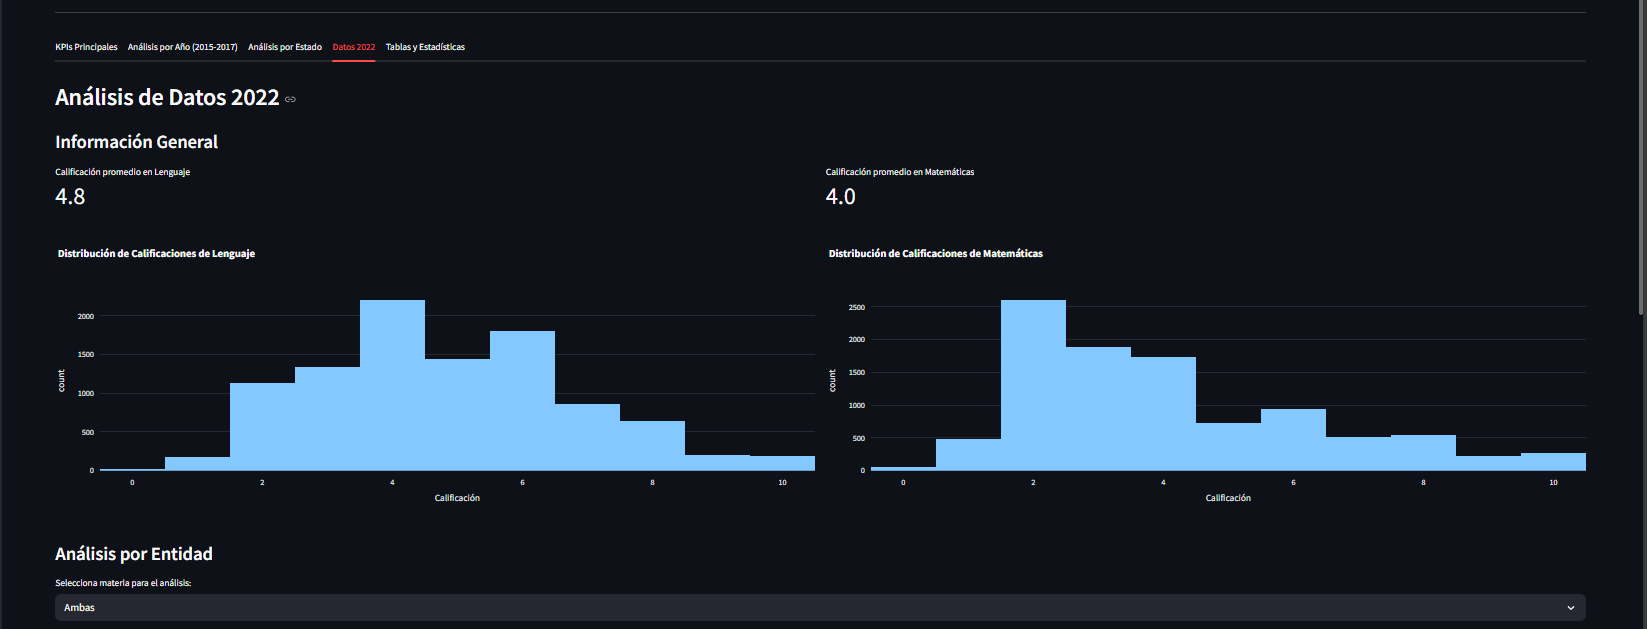
\includegraphics[width=0.8\textwidth]{../imagenes/analisis 2022.png}
    \caption{Ejemplo de histograma en el dashboard para datos 2022}
    \label{fig:histograma}
\end{figure}

\subsection{Gráficos de Correlación}
Para análisis de relaciones entre variables, se implementaron matrices de correlación:

\begin{lstlisting}[language=Python, caption=Implementación de matrices de correlación]
# Seleccionar variables numéricas para correlación
variables_seleccionadas = st.multiselect("Selecciona variables para la correlación:", 
                                        [col for col in df_año.columns if df_año[col].dtype in ['int64', 'float64']])

if variables_seleccionadas:
    # Calcular matriz de correlación
    corr_matrix = df_año[variables_seleccionadas].corr()
    
    # Visualizar como heatmap
    fig = px.imshow(
        corr_matrix,
        text_auto=True,
        aspect="auto",
        color_continuous_scale="RdBu_r",
        title=f"Matriz de correlación para variables seleccionadas ({anio_seleccionado})"
    )
    st.plotly_chart(fig, use_container_width=True)
\end{lstlisting}

Beneficios de esta visualización:
\begin{itemize}
    \item Identificación de relaciones entre variables educativas
    \item Descubrimiento de patrones no evidentes en análisis univariados
    \item Base para análisis más profundos de causalidad
\end{itemize}

\begin{figure}[h]
    \centering
    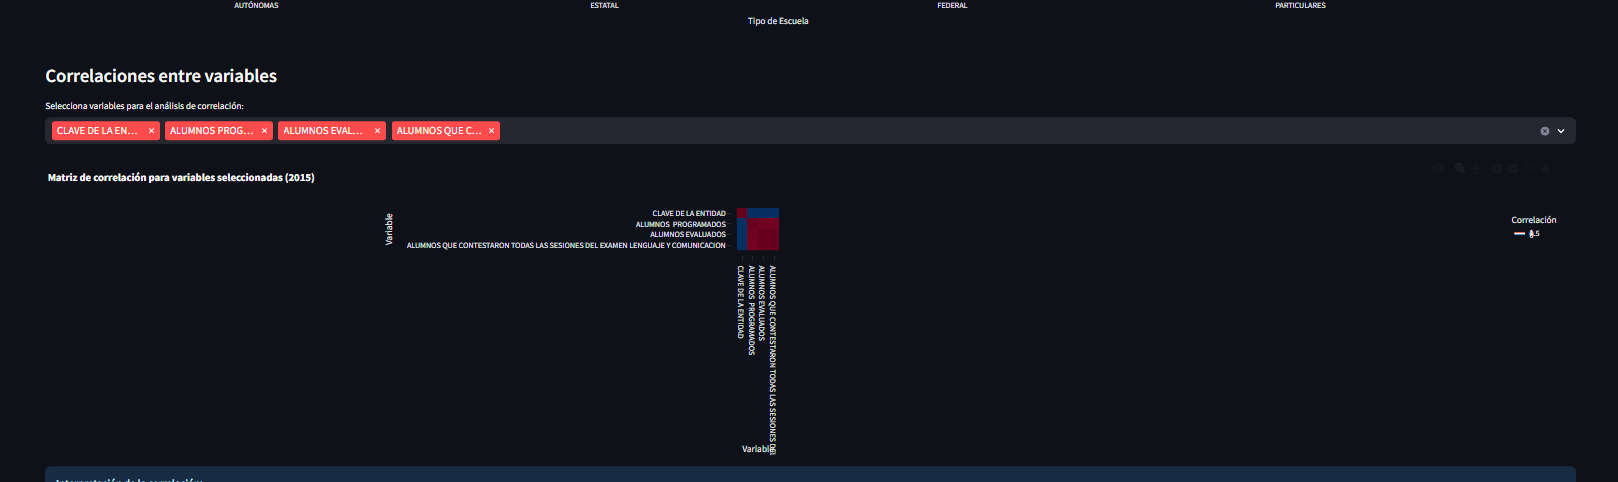
\includegraphics[width=0.8\textwidth]{../imagenes/correlaciones entre variables.png}
    \caption{Ejemplo de matriz de correlación en el dashboard}
    \label{fig:matriz_correlacion}
\end{figure}

\subsection{Tablas Interactivas}
Las tablas interactivas permiten explorar datos detallados:

\begin{lstlisting}[language=Python, caption=Implementación de tablas interactivas]
# Función para destacar filas
def highlight_row(row):
    if row["Entidad"] == entidad_seleccionada:
        return ['background-color: #FFFF00'] * len(row)
    return [''] * len(row)

# Aplicar estilo y mostrar
df_ranking_display = df_ranking.style.apply(highlight_row, axis=1)
st.dataframe(df_ranking_display[["Posición", "Entidad", "Porcentaje"]], height=400)
\end{lstlisting}

Características implementadas:
\begin{itemize}
    \item Ordenamiento dinámico por columnas
    \item Resaltado de filas relevantes
    \item Paginación para grandes conjuntos de datos
    \item Filtrado interactivo
\end{itemize}

\begin{figure}[h]
    \centering
    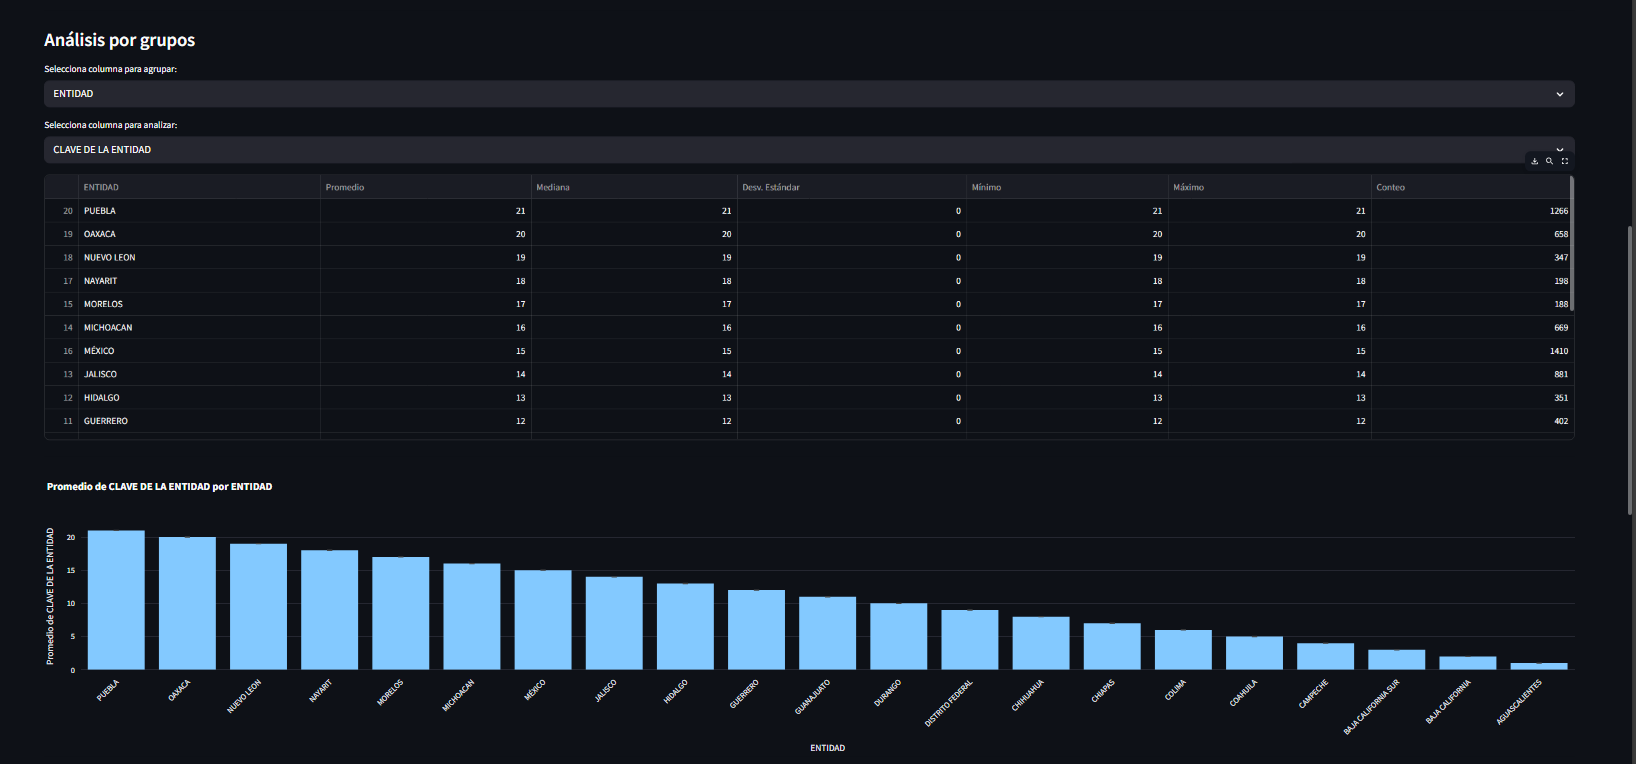
\includegraphics[width=0.8\textwidth]{../imagenes/analisis por gruoi.png}
    \caption{Ejemplo de tabla interactiva en el dashboard}
    \label{fig:tabla_interactiva}
\end{figure}

\subsection{Control de Carga de Datos}
Para optimizar el rendimiento del dashboard, especialmente con grandes volúmenes de datos, se implementó un sistema de control de carga.

\begin{figure}[h]
    \centering
    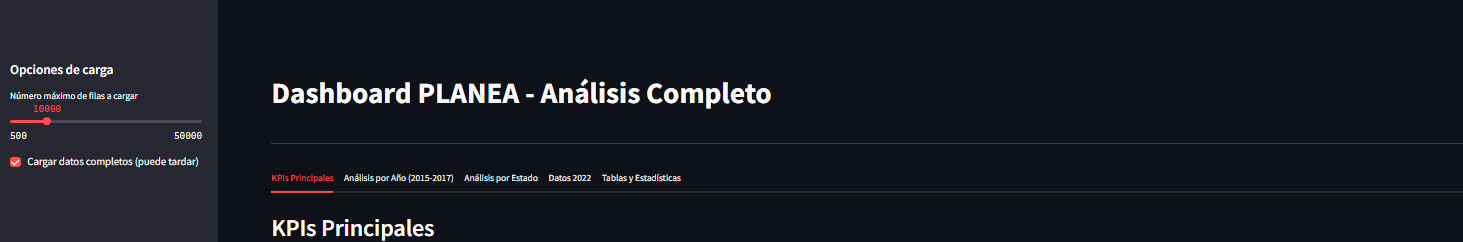
\includegraphics[width=0.8\textwidth]{../imagenes/opciones de carga.png}
    \caption{Opciones de control para la carga de datos en el dashboard}
    \label{fig:opciones_carga}
\end{figure}

\subsection{Pestaña 3: Análisis por Estado}
Dedicada al análisis geográfico:

\begin{itemize}
    \item \textbf{Evolución de la entidad}: Gráfico de línea mostrando tendencias para la entidad seleccionada.
    
    \item \textbf{Comparativa con el promedio nacional}: Contraste entre la entidad seleccionada y la media nacional.
    
    \item \textbf{Ranking nacional}: Tabla que muestra la posición relativa de cada entidad.
\end{itemize}

\begin{figure}[h]
    \centering
    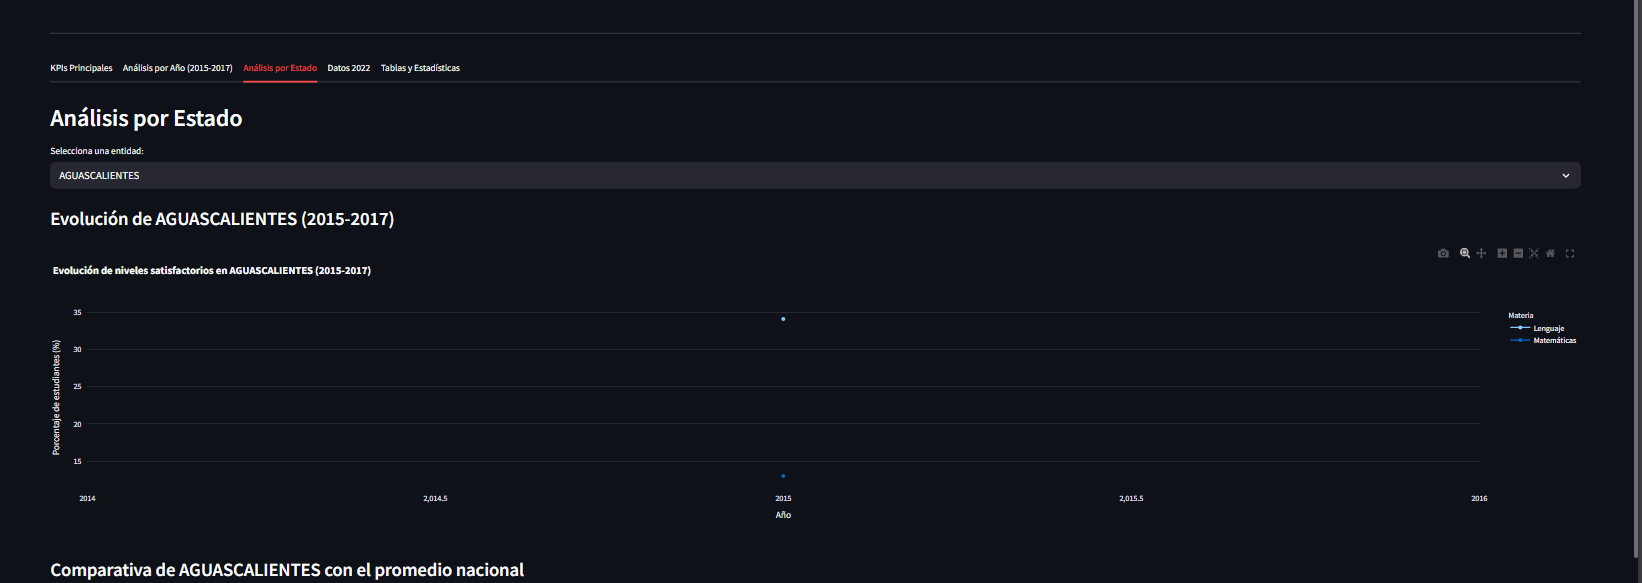
\includegraphics[width=0.8\textwidth]{../imagenes/ananlisis por estado .png}
    \caption{Análisis por estado mostrando comparativas y rankings}
    \label{fig:analisis_estado}
\end{figure}

\begin{figure}[h]
    \centering
    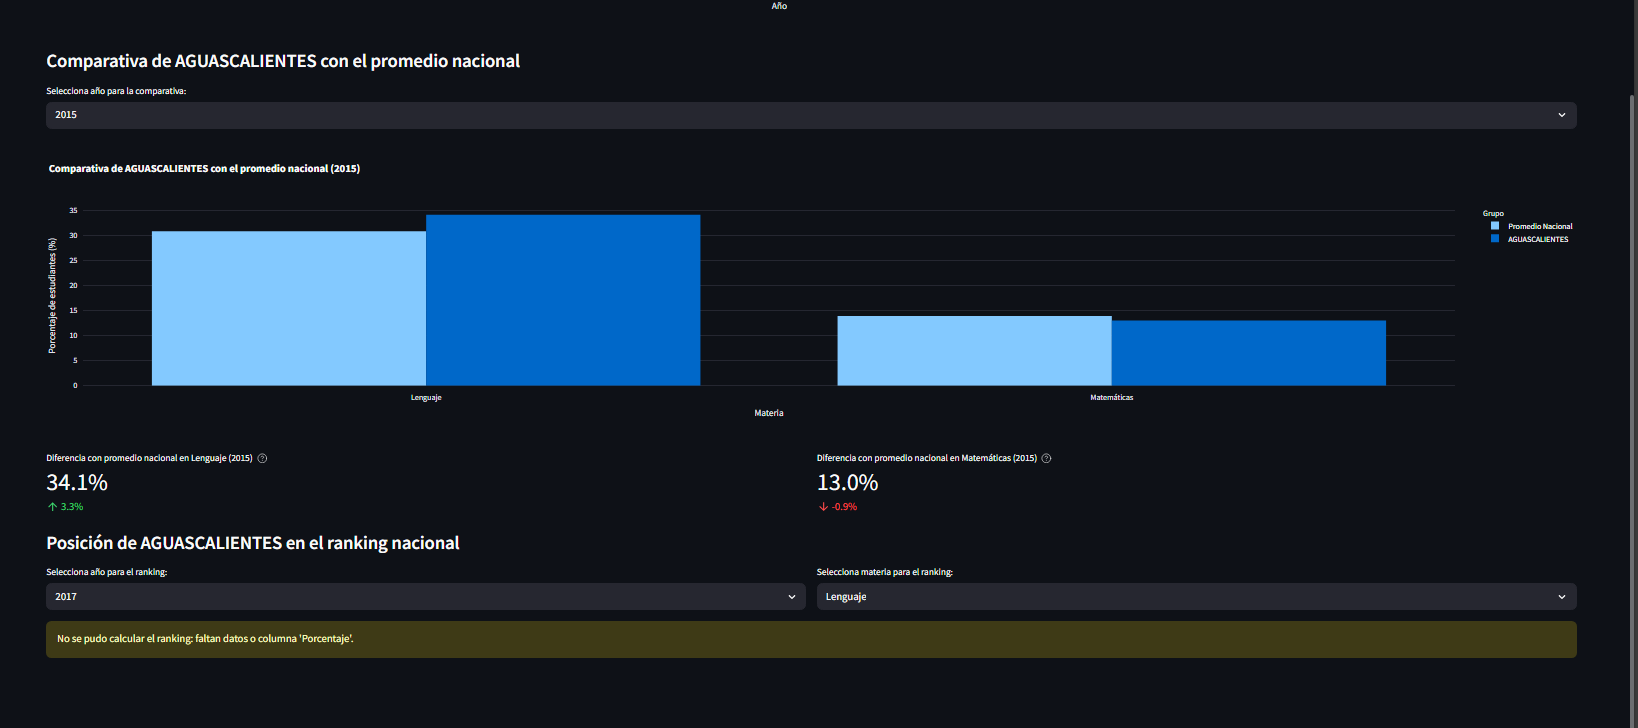
\includegraphics[width=0.8\textwidth]{../imagenes/comparativa con promedio nacioanal.png}
    \caption{Comparativa del desempeño de entidades con el promedio nacional}
    \label{fig:comparativa_nacional}
\end{figure}

\subsection{Pestaña 4: Datos 2022}
Enfocada en los datos más recientes:

\begin{itemize}
    \item \textbf{Información general}: Calificaciones promedio en Lenguaje y Matemáticas.
{{ ... }}
    \item \textbf{Análisis por entidad}: Gráficos de barras comparando entidades.
    \item \textbf{Nota comparativa}: Advertencia sobre las limitaciones de comparabilidad con años anteriores.
\end{itemize}

\begin{figure}[h]
    \centering
    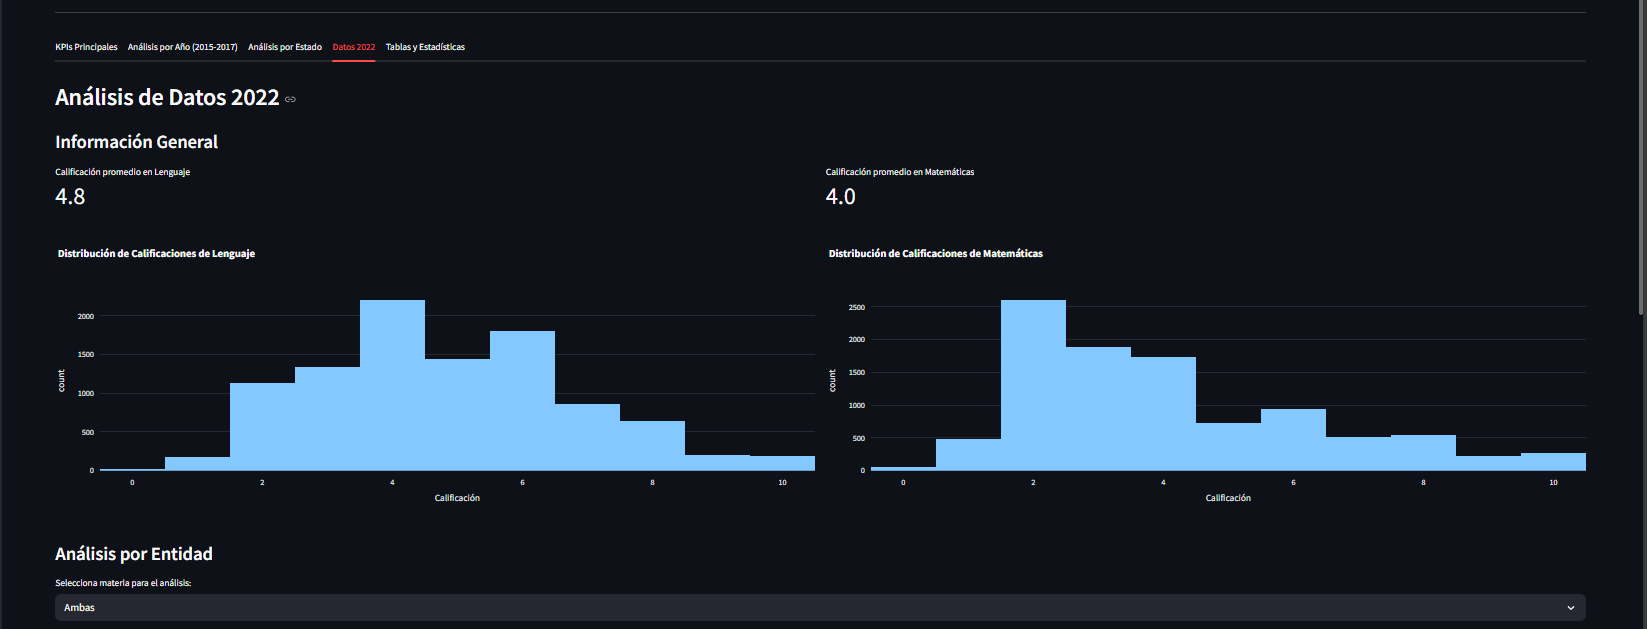
\includegraphics[width=0.8\textwidth]{../imagenes/analisis 2022.png}
    \caption{Distribución de calificaciones en Lenguaje y Matemáticas (2022)}
    \label{fig:histograma_2022}
\end{figure}

\subsection{Pestaña 5: Tablas y Estadísticas}
Proporciona acceso a datos más detallados:

\begin{itemize}
    \item \textbf{Previsualizaciones de datos}: Tablas mostrando las primeras filas de cada conjunto de datos.
    \item \textbf{Estadísticas descriptivas}: Resúmenes estadísticos calculados con \texttt{df.describe()}.
    \item \textbf{Análisis por grupos}: Estadísticas agrupadas por variables seleccionadas.
    \item \textbf{Filtrado personalizado}: Herramientas para crear subconjuntos específicos.
\end{itemize}

\begin{figure}[h]
    \centering
    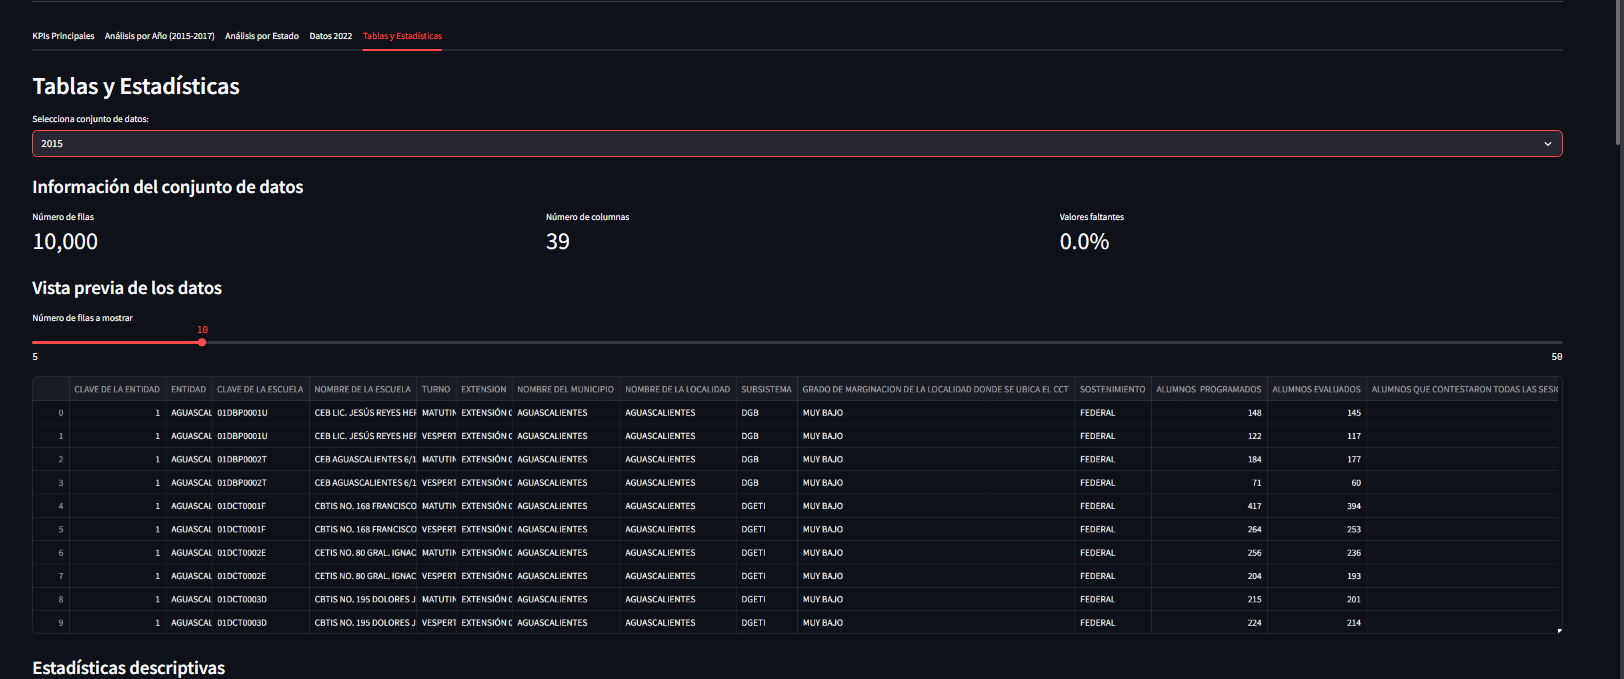
\includegraphics[width=0.8\textwidth]{../imagenes/tabla y estadisticas.png}
    \caption{Tablas y estadísticas descriptivas de los datos}
    \label{fig:tablas_estadisticas}
\end{figure}

\begin{figure}[h]
    \centering
    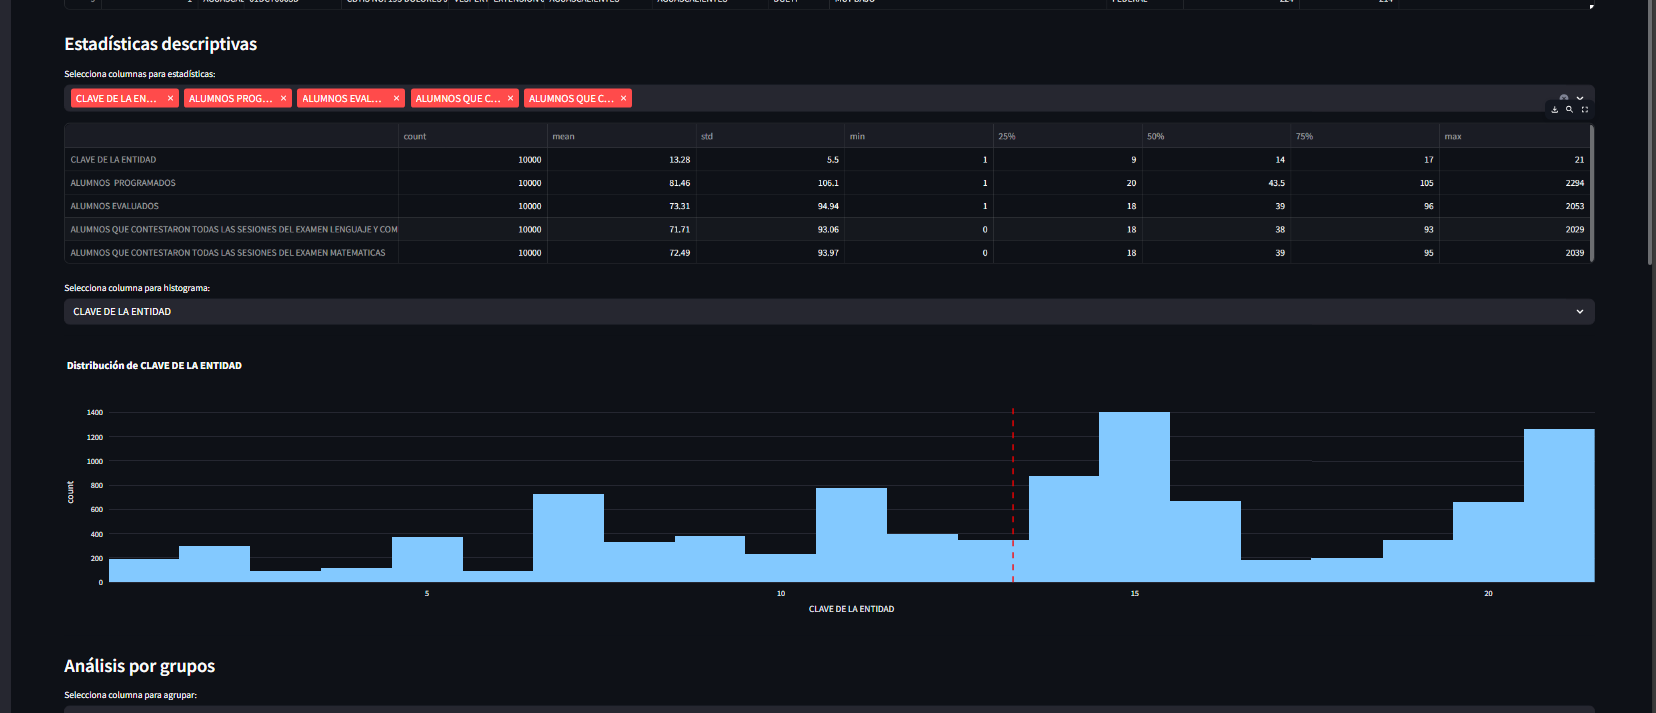
\includegraphics[width=0.8\textwidth]{../imagenes/estadisticas descripticas.png}
    \caption{Resúmenes estadísticos detallados de las variables numéricas}
    \label{fig:estadisticas_descriptivas}
\end{figure}

\section{Interactividad y Filtros}

\begin{figure}[h]
    \centering
    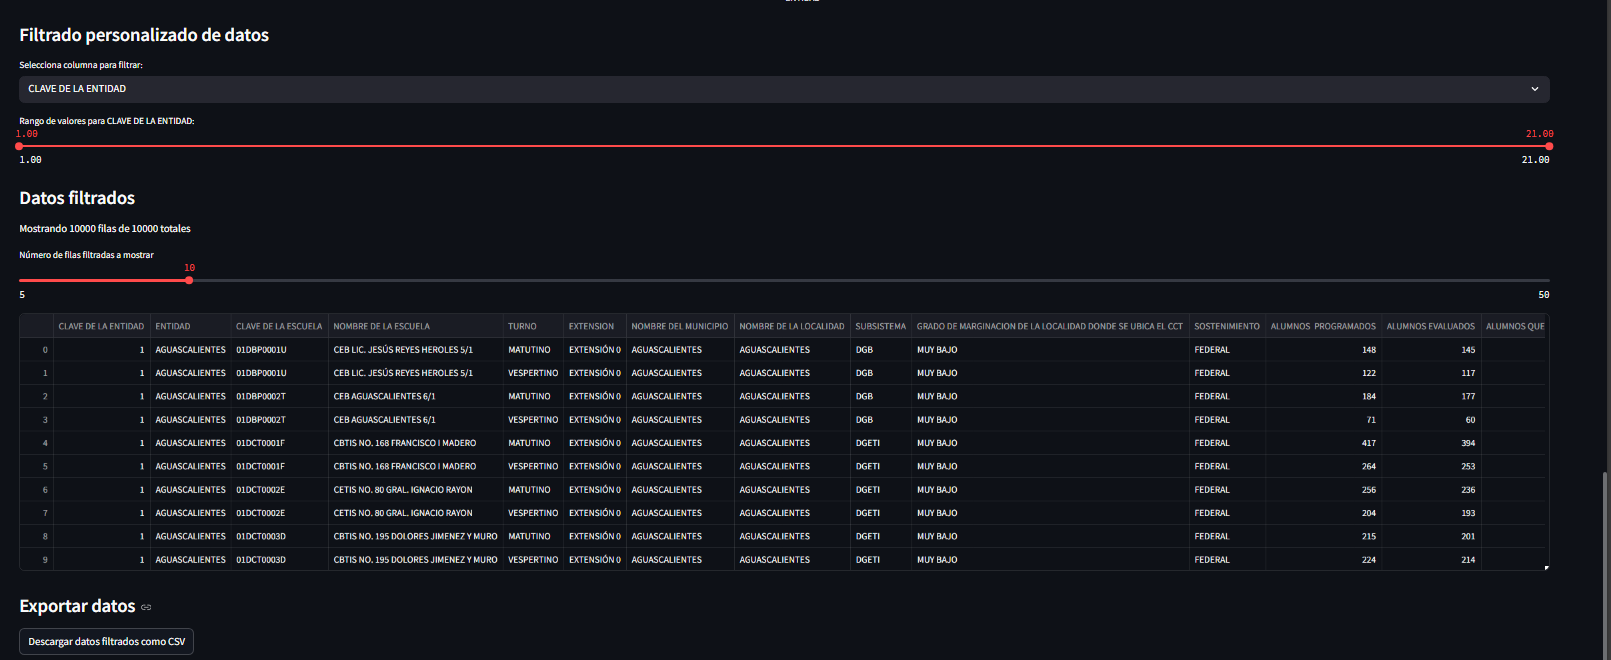
\includegraphics[width=0.8\textwidth]{../imagenes/filtrado de datos.png}
    \caption{Opciones de filtrado interactivo en el dashboard}
    \label{fig:filtrado_datos}
\end{figure}

\subsection{Selectores Implementados}
El dashboard incorpora diversos elementos interactivos:

\begin{lstlisting}[language=Python, caption=Implementación de selectores]
# Selector de año
anio_seleccionado = st.selectbox("Selecciona un año para analizar:", [2015, 2016, 2017])

# Selector de tipo de escuela
tipo_escuela = st.selectbox("Selecciona un tipo de escuela:", ["AUTÓNOMAS", "ESTATAL", "FEDERAL", "PARTICULARES"])

# Selector de entidad
entidad_seleccionada = st.selectbox("Selecciona una entidad:", entidades)

# Selector múltiple para variables
variables = st.multiselect("Selecciona variables para el análisis:", columnas_numericas)
\end{lstlisting}

\subsection{Filtros Dinámicos}
Los filtros se implementan de forma dinámica:

\begin{lstlisting}[language=Python, caption=Implementación de filtros dinámicos]
# Filtro por entidad
df_filtrado = df[df[entidad_col] == entidad_seleccionada]

# Filtro por año
df_filtrado = df[df["AÑO"] == anio_seleccionado]

# Filtro por tipo de escuela
df_filtrado = df[df["TIPO DE ESCUELA"] == tipo_escuela]

# Filtro personalizado con slider
valor_minimo = st.slider("Filtrar por valor mínimo:", 
                         min_value=float(df[columna].min()), 
                         max_value=float(df[columna].max()))
df_filtrado = df[df[columna] >= valor_minimo]
\end{lstlisting}

\subsection{Elementos Interactivos en Visualizaciones}
Las visualizaciones incluyen elementos interactivos avanzados:

\begin{itemize}
    \item \textbf{Tooltips}: Información detallada al pasar el cursor sobre elementos gráficos.
    \item \textbf{Zoom}: Capacidad para ampliar áreas específicas de los gráficos.
    \item \textbf{Selección}: Posibilidad de seleccionar elementos específicos para análisis detallado.
    \item \textbf{Leyendas interactivas}: Clic en leyendas para mostrar/ocultar series.
    \item \textbf{Botones de descarga}: Opción para guardar gráficos como imágenes.
\end{itemize}

\section{Personalización Visual}

\subsection{Paleta de Colores}
Se implementó una paleta de colores consistente:

\begin{itemize}
    \item \textbf{Colores primarios}: Azul claro y azul oscuro para las dos materias principales.
    \item \textbf{Colores de contraste}: Rojo y verde para indicadores de cambio.
    \item \textbf{Colores neutros}: Grises para elementos secundarios.
    \item \textbf{Destacados}: Amarillo para resaltar elementos seleccionados.
\end{itemize}

\subsection{Temas y Estilos}
El dashboard utiliza un tema oscuro para mejorar la legibilidad y reducir la fatiga visual:

\begin{lstlisting}[language=Python, caption=Configuración de tema]
# Tema oscuro predeterminado en Streamlit
# Personalización adicional de elementos
st.markdown("""
<style>
    .metric-label { font-size: 0.8rem !important; }
    .metric-value { font-weight: bold !important; }
    .warning { background-color: rgba(255, 190, 0, 0.2); padding: 10px; border-radius: 5px; }
</style>
""", unsafe_allow_html=True)
\end{lstlisting}

\section{Accesibilidad y Usabilidad}

\subsection{Consideraciones de Accesibilidad}
Se implementaron diversas características para mejorar la accesibilidad:

\begin{itemize}
    \item \textbf{Contraste adecuado}: Asegurar legibilidad para personas con baja visión.
    \item \textbf{Textos alternativos}: Descripciones para elementos visuales.
    \item \textbf{Paleta amigable para daltonismo}: Selección de colores distinguibles por personas con daltonismo.
    \item \textbf{Estructura jerárquica}: Organización lógica para lectores de pantalla.
\end{itemize}

\subsection{Mejoras de Usabilidad}
Para optimizar la experiencia de usuario:

\begin{itemize}
    \item \textbf{Mensajes de ayuda}: Tooltips y explicaciones sobre funcionalidades.
    \item \textbf{Retroalimentación visual}: Indicadores claros de estados y acciones.
    \item \textbf{Consistencia}: Patrones de interacción similares en todo el dashboard.
    \item \textbf{Mensajes de error informativos}: Comunicación clara cuando algo no funciona.
\end{itemize}

\section{Desafíos y Soluciones}

\subsection{Visualización de Datos Incompletos}
Para manejar datos faltantes en las visualizaciones:

\begin{itemize}
    \item \textbf{Advertencias visuales}: Mensajes claros cuando faltan datos.
    \item \textbf{Visualizaciones adaptativas}: Gráficos que se ajustan a datos parciales.
    \item \textbf{Indicadores de completitud}: Información sobre qué porcentaje de datos está disponible.
\end{itemize}

\subsection{Comparabilidad Visual entre Períodos}
Para abordar los desafíos de visualización entre datos 2015-2017 y 2022:

\begin{itemize}
    \item \textbf{Etiquetas diferenciadoras}: Distinción clara entre porcentajes y calificaciones promedio.
    \item \textbf{Escalas separadas}: Uso de ejes diferentes cuando es necesario.
    \item \textbf{Notas contextuales}: Información clara sobre cambios metodológicos.
    \item \textbf{Visualizaciones paralelas}: Presentación lado a lado en lugar de superpuesta cuando es apropiado.
\end{itemize}

\section{Evaluación de Efectividad}

\subsection{Criterios de Evaluación}
Las visualizaciones fueron evaluadas según los siguientes criterios:

\begin{itemize}
    \item \textbf{Precisión}: Representación fiel de los datos subyacentes.
    \item \textbf{Claridad}: Facilidad de comprensión para usuarios diversos.
    \item \textbf{Eficiencia}: Cantidad de información transmitida por unidad de espacio.
    \item \textbf{Contextualización}: Presencia de elementos que facilitan la interpretación.
    \item \textbf{Estética}: Atractivo visual sin comprometer la funcionalidad.
\end{itemize}

\subsection{Mejoras Iterativas}
El diseño visual evolucionó a través de un proceso iterativo:

\begin{itemize}
    \item \textbf{Revisión de literatura}: Incorporación de mejores prácticas de visualización de datos educativos.
    \item \textbf{Pruebas con usuarios}: Ajustes basados en retroalimentación de usuarios potenciales.
    \item \textbf{Análisis de interacción}: Optimización basada en patrones de uso observados.
    \item \textbf{Refinamiento técnico}: Mejoras en rendimiento y precisión de visualizaciones.
\end{itemize}

En conclusión, las visualizaciones implementadas en el dashboard PLANEA representan un balance entre rigor analítico, claridad comunicativa y usabilidad, permitiendo a usuarios con diferentes niveles de experiencia extraer información valiosa sobre el desempeño educativo en México a través de los años evaluados.
